%%%%%%%%%%%%%%%%%%%%%%%%%%%%%%%%%%%%%%%%%%%%%%%%%%%
%
%  New template code for TAMU Theses and Dissertations starting Fall 2012.  
%  For more info about this template or the 
%  TAMU LaTeX User's Group, see http://www.howdy.me/.
%
%  Author: Wendy Lynn Turner 
%
%%%%%%%%%%%%%%%%%%%%%%%%%%%%%%%%%%%%%%%%%%%%%%%%%%%

\documentclass[12pt]{report}
\usepackage[letterpaper]{geometry}
\geometry{verbose,tmargin=1.25in,bmargin=1.25in,lmargin=1.4in,rmargin=1.15in}
 \usepackage[doublespacing]{setspace}
 \usepackage{tocloft}
 \usepackage[rm, tiny,center, compact]{titlesec}
 \usepackage{indentfirst}
 \usepackage{etoolbox}
\usepackage{tocvsec2}
 \usepackage[titletoc]{appendix}
 \usepackage{appendix}
 \usepackage{tamuconfig}
\usepackage{rotating}

% Added to fix issues with pdf searching in some versions of LaTeX
%\usepackage[T1]{fontenc}\usepackage{lmodern}
%%%%%%%%%%%%%%%%%%%%%%%%%%%%%

% Hyperref setup below.  You should be able to get away with using uncommenting just the first line.
%\usepackage[hidelinks]{hyperref}

% if \usepackage[hidelinks]{hyperref} doesn't work try this.
% \usepackage{hyperref}  % Hidelinks is an option that removes link visiability.  TAMU Thesis Offices prefers to not see the links. But often doesn't work.  
% 
% \hypersetup{
%     colorlinks=true,
%     linkcolor=black,
%     citecolor=black,
%     filecolor=black,
%     urlcolor=black,
% }
%%%%%%%  End of hyperref setup.  One of these two options should work, but my motto with hyperref is when in doubt, comment it out!
%%%%%%%%%  This hopefully fixes the problem with vertical spacing of section headings at the top of the page..  Commented out in 1.0.7
% \preto\section{%
% \ifnum\value{section}>0\addtocontents{toc}{\vskip-6pt}\fi
% }
% \preto\subsection{%
% \ifnum\value{subsection}=0\addtocontents{toc}{\vskip-6pt}\fi
% \ifnum\value{subsection}>0\addtocontents{toc}{\vskip-6pt}\fi
% } 
%%%%%%%%%%%%%%%%%%%%%%%%%%%%%%%%%%%%%%%%%%%%%%%%%%%%%%

\begin{document}

\renewcommand{\tamumanuscripttitle}{Type in your default title here: You may need to change the spacing if the title is too long and pushes the copyright off of the titlepage }
\renewcommand{\tamupapertype}{Dissertation}
\renewcommand{\tamufullname}{First Middle Lastname}
\renewcommand{\tamudegree}{Doctor of Philosophy}
\renewcommand{\tamuchairone}{Chair Name}
% Uncomment out the next line if you have co-chairs.  You will also need to edit the titlepage.tex file.
%\newcommand{\tamuchairtwo}{Additional Chair Name}
\renewcommand{\tamumemberone}{Committee Member1}
\newcommand{\tamumembertwo}{Committee Member2}
\newcommand{\tamumemberthree}{Committee Member3}
\renewcommand{\tamudepthead}{Head of Department}
\renewcommand{\tamugradmonth}{December}
\renewcommand{\tamugradyear}{2012}
\renewcommand{\tamudepartment}{Department Name}


%%%%%%%%%%%%%%%%%%%%%%%%%%%%%%%%%%%%%%%%%%%%%%%%%%%
%
%  New template code for TAMU Theses and Dissertations starting Fall 2012.  
%  For more info about this template or the 
%  TAMU LaTeX User's Group, see http://www.howdy.me/.
%
%  Author: Wendy Lynn Turner 
%	 Version 1.0 
%  Last updated 8/5/2012
%
%%%%%%%%%%%%%%%%%%%%%%%%%%%%%%%%%%%%%%%%%%%%%%%%%%%

%%%%%%%%%%%%%%%%%%%%%%%%%%%%%% 
%% TITLE PAGE
%% The values get updated automatically.  Please do not make changes to this file other than adding/deleting committee members where necessary.
%%%%%%%%%%%%%%%%%%%%%%%%%%%%%%

\providecommand{\tabularnewline}{\\}



\begin{titlepage}
\begin{center}
\MakeUppercase{\tamumanuscripttitle}
\vspace{4em}

A \tamupapertype

by

\MakeUppercase{\tamufullname}

\vspace{4em}

\begin{singlespace}

Submitted to the Office of Graduate and Professional Studies of \\
Texas A\&M University \\

in partial fulfillment of the requirements for the degree of \\
\end{singlespace}

\MakeUppercase{\tamudegree}
\par\end{center}
\vspace{2em}
\begin{singlespace}
\begin{tabular}{ll}
 & \tabularnewline
& \cr
% If you have Co-Chairs comment out the 'Chair of Committee' line below and uncomment the 'Co-Chairs of Committee' line.
Chair of Committee, & \tamuchairone\tabularnewline
%Co-Chairs of Committee, & \tamuchairone\tabularnewline & \tamuchairtwo\tabularnewline
Committee Members, & \tamumemberone\tabularnewline
 & \tamumembertwo\tabularnewline
 & \tamumemberthree\tabularnewline
Head of Department, & \tamudepthead\tabularnewline

\end{tabular}
\end{singlespace}
\vspace{3em}

\begin{center}
\tamugradmonth \hspace{2pt} \tamugradyear

\vspace{3em}

Major Subject: \tamudepartment \par
\vspace{3em}
Copyright \tamugradyear \hspace{.5em}\tamufullname 
\par\end{center}
\end{titlepage}
\pagebreak{}




 % This is simply a file that formats and adds your titlepage, please do not edit this unless you have a specific need. .
%%%%%%%%%%%%%%%%%%%%%%%%%%%%%%%%%%%%%%%%%%%%%%%%%%%
%
%  New template code for TAMU Theses and Dissertations starting Fall 2016.  
%
%
%  Author: Sean Zachary Roberson
%  Version 3.17.06
%  Last Updated: 6/15/2017
%
%%%%%%%%%%%%%%%%%%%%%%%%%%%%%%%%%%%%%%%%%%%%%%%%%%%
%%%%%%%%%%%%%%%%%%%%%%%%%%%%%%%%%%%%%%%%%%%%%%%%%%%%%%%%%%%%%%%%%%%%%
%%                           ABSTRACT 
%%%%%%%%%%%%%%%%%%%%%%%%%%%%%%%%%%%%%%%%%%%%%%%%%%%%%%%%%%%%%%%%%%%%%

\chapter*{ABSTRACT}
\addcontentsline{toc}{chapter}{ABSTRACT} % Needs to be set to part, so the TOC doesnt add 'CHAPTER ' prefix in the TOC.

\pagestyle{plain} % No headers, just page numbers
\pagenumbering{roman} % Roman numerals
\setcounter{page}{2}

\indent The broad theme of this work is the application of iterative algorithms, that closely resemble peeling decoder in the overall philosophy, to problems that are enormous in scale but whose actual parameters of interest are sparse in nature. Specifically this thesis focuses on the massive multiple access, compressed sensing and group testing problems. In all of these problems the total number of parameters are very large, where the parameters for the respective problems correspond to the number of users present in the system, the length of the signal to be compressed and the number of items that are to be tested for defects. However, the number of actual parameters of interest are fairly small in comparison, where the parameters of interest in the respective problems correspond to the number of users that are active at any given time, the number of dimensions with significant signal power and the number of defective items present. The proposed design schemes attempt to explore this sparse nature of the parameters of interest. The main components common to all the proposed schemes are: (i) A variant of a sparse bipartite Tanner graph is used as the basis for designing the interaction strategy between the parameters of interest (ii) An iterative algorithm similar to peeling decoder is used for recovering those parameters of interest. Both these tools are popular in channel coding literature \cite{richardson2008modern} but are not as widely used in the respective areas of study and this thesis is a step in that direction to bridge the gap.

The contributions of this thesis can be categorized into four parts:
\begin{enumerate}
\item The first part considers the unsourced version of the massive multiple access problem, which will be referred to as unsourced MAC. In the unsourced MAC problem setup, a large number of devices are present in the system where each device has a brief message to communicate to a central receiver sporadically. Distinguishing from the traditional MAC is the fact that the receiver is interested only in the set of messages transmitted and disinterested in the source of the respective messages thus the term \textit{unsourced}. Due to the sporadic nature of the data to be transmitted, the number of active devices at any particular time is fairly small. The main components of the proposed coding scheme for the unsourced MAC are: (i) The transmitted message consists of two parts. The first part chooses an interleaver for a low density parity check (LDPC) type code. For encoding the first part, a code that is designed to be decoded efficiently by a compressed sensing type decoder is chosen (ii) The second part of the message is encoded by the LDPC code for which the interleaver is chosen by the first part of the message. A joint message passing type decoder designed for the T-user binary input real adder channel is used to decode the interfering LDPC codewords at each slot. (iii) Each user repeats the transmitted codeword in multiple time slots where the repetition pattern is determined solely by the message being encoded. Thus this scheme is amenable to a successive interference cancellation decoder where a codeword decoded at any one slot can be removed  (\textit{peeling-off}) from all other slots it was transmitted in. This coding scheme improves upon the practical coding scheme introduced by Ordentlich and Polyanskiy in \cite{ordentlich2017low} which is the best when compared to the other multiple access solutions available in literature such as treat interference as noise (TIN) and slotted-ALOHA. The proposed coding scheme is only $\approx 6$dB away from the achievable limit based on random Gaussian coding and the ideal joint typical decoder which has exponential complexity and is impractical.
The unsourced MAC is followed by the consideration of uncoordinated MAC problem wherein no power constraints are imposed on the individual users. In the non-asymptotic case i.e. when the number of users is fixed and finite, an analytic expression is found to compute the error performance of the successive interference cancellation scheme as a function of the random access strategy employed by each user. The analytic expression proposed is verified to be accurate through simulations. This provides a possible solution path, using gradient ascent approach, to derive a random access strategy that is optimal in terms of the total throughput achievable.

\item In the second part, the design of construction-D lattices for the interference channel is considered. The proposed construction scheme uses spatially-coupled low-density parity check (LDPC) codes \cite{felstrom1999time,kudekar2011threshold}. The fact that these codes achieve the channel capacity on the class of binary memory-less symmetric channels is leveraged to achieve the Poltyrev limit for lattices. The lattice codes derived from this class of lattices are shown to provide excellent performance for the symmetric Gaussian interference channel. The simulation results demonstrate that the proposed lattice codes under the low-complexity multistage belief propagation decoder can perform within 1.02dB (discounting the 1.53dB shaping loss) of the Shannon limit for the symmetric interference channel 

\item The third part considers the design of a family of sensing matrices for the problem of support recovery in compressed sensing. In the proposed design scheme the sensing matrix when represented using graph structure has a close resemblance to the left and right regular LDPC codes. An iterative algorithm similar to the peeling decoder is employed for the recovery of the sparse signal. The proposed design scheme enables to achieve the number of measurements and decoding complexity that match the best possible lower bounds upto a constant.% that are order optimal in the number of measurements and decoding complexity.
  

\item In the fourth part testing schemes for the non-adaptive group testing problem are considered. Similar to the compressed sensing, the testing scheme resembles left and right regular bipartite graph in structure and the algorithm for recovering the defective items is similar to a peeling decoder. With the proposed testing scheme the number of tests required is order optimal and more importantly the recovery algorithm has only a sub-linear time complexity.
\end{enumerate} 
\pagebreak{}

%%%%%%%%%%%%%%%%%%%%%%%%%%%%%%%%%%%%%%%%%%%%%%%%%%%
%
%  New template code for TAMU Theses and Dissertations starting Fall 2016.  
%
%
%  Author: Sean Zachary Roberson
%  Version 3.17.06
%  Last Updated: 6/15/2017
%
%%%%%%%%%%%%%%%%%%%%%%%%%%%%%%%%%%%%%%%%%%%%%%%%%%%

%%%%%%%%%%%%%%%%%%%%%%%%%%%%%%%%%%%%%%%%%%%%%%%%%%%%%%%%%%%%%%%%%%%%%%
%%                           DEDICATION
%%%%%%%%%%%%%%%%%%%%%%%%%%%%%%%%%%%%%%%%%%%%%%%%%%%%%%%%%%%%%%%%%%%%%
%\chapter*{DEDICATION}
\addcontentsline{toc}{chapter}{DEDICATION}  % Needs to be set to part, so the TOC doesnt add 'CHAPTER ' prefix in the TOC.



\begin{center}
\vspace*{\fill}
To my loving family,\\
and in memory of my uncle (1964-2014)
\vspace{6in}
\end{center}

\pagebreak{}

%%%%%%%%%%%%%%%%%%%%%%%%%%%%%%%%%%%%%%%%%%%%%%%%%%%
%
%  New template code for TAMU Theses and Dissertations starting Fall 2016.  
%
%
%  Author: Sean Zachary Roberson
%  Version 3.17.06
%  Last Updated: 6/15/2017
%
%%%%%%%%%%%%%%%%%%%%%%%%%%%%%%%%%%%%%%%%%%%%%%%%%%%


%%%%%%%%%%%%%%%%%%%%%%%%%%%%%%%%%%%%%%%%%%%%%%%%%%%%%%%%%%%%%%%%%%%%%%
%%                           ACKNOWLEDGMENTS
%%%%%%%%%%%%%%%%%%%%%%%%%%%%%%%%%%%%%%%%%%%%%%%%%%%%%%%%%%%%%%%%%%%%%
\chapter*{ACKNOWLEDGMENTS}
\addcontentsline{toc}{chapter}{ACKNOWLEDGMENTS}  % Needs to be set to part, so the TOC doesnt add 'CHAPTER ' prefix in the TOC.

It was a long, rewarding and fulfilling journey to my Ph. D. degree. This would not have been possible if not for the support and encouragement of a lot of people starting from my teachers and friends in high school to my professors, friends and colleagues at Texas A\&M university. My heartfelt gratitude and thanks go out to each and everyone who helped me and stood by me.

\indent First and foremost, I would like to thank my advisor Dr. Krishna Narayanan for his guidance throughout the past six years of my graduate studies. He was always available, literally a knock-on-the-door away, with plenty of time for me. I will be forever indebted to his teachings, support and the valuable directions he provided in times of struggle. He taught me coding and information theory courses in my first two semesters at Texas A\& M University and his passionate teaching arose the curiosity in me and laid the foundations for my subsequent forays into these rich and beautiful areas of research. I am truly fortunate to have spent the formative years of my academic and professional career under the tutelage of such a wonderful academic and a warm person. I hope to carry his legacy forward.

I would like to thank Professors Jean-Francois Chamberland, Arun Srinivasa, and Alex Sprintson for their time in serving on my thesis committee. I am thankful for their insights.

I am thankful to a lot of friends and colleagues whose company and camaraderie made this journey all the more enjoyable. I want to reminisce and thank my roommates Nilu, Rhushabh `Sir' for all the late night discussions, Shweta, Suraj, Sneha, Gupta \textit{et al}., from my second-family `Nagle' group for the innumerable weekends spent in laughter and banter, Manjusha, Kartheek and Siddhitha for their affection. I am also thankful to my lab-mates Arvind Yedla, for the crazy parties and fun times spent in and `around' Eugenes, Santhosh Vanaparthy, for the hours long discussions we had on a wide range of topics varying from madness of mathematicians like Paul Dirac to the importance/stupidity of sports etc., Rahul, Emmadi, Jerry Huang, Engin, Yung-Yih Jian, Fatemeh, Nagaraj, Paul, Arman, and several others.

Above all, I am forever grateful to Dakshna for all the wonderful times we spent in College Station, for being with me in the ups and downs of this journey, for providing the care, comfort, motivation, encouragement, guidance and support when I needed them. At a moment of looking back, I want to remember my uncle Narasimha Reddy for his assistance and encouragement in my pursuing higher studies. Although no longer with us, he continues to inspire me by the hard work and love he showed for his family.

Finally, I express my deepest gratitude to my parents, Ranga Reddy and Andalamma, and my little sister Anu for their unconditional love and support and for the immense faith they have always shown in me. I cannot thank enough, my mother for all the sacrifices she made to ensure our happiness, and my father for engaging me in all my inane questions in my childhood, his insistence that I learn the mathematics and the sciences in the \textit{right} way and for prioritizing the higher education of me and my sister above all else. I will be forever indebted to them.
\pagebreak{}
%%%%%%%%%%%%%%%%%%%%%%%%%%%%%%%%%%%%%%%%%%%%%%%%%%%
%
%  New template code for TAMU Theses and Dissertations starting Fall 2016.  
%
%
%  Author: Sean Zachary Roberson
%  Version 3.17.06
%  Last Updated: 6/15/2017
%
%%%%%%%%%%%%%%%%%%%%%%%%%%%%%%%%%%%%%%%%%%%%%%%%%%%

%%%%%%%%%%%%%%%%%%%%%%%%%%%%%%%%%%%%%%%%%%%%%%%%%%%%%%%%%%%%%%%%%%%%%%
%%                           NOMENCLATURE
%%%%%%%%%%%%%%%%%%%%%%%%%%%%%%%%%%%%%%%%%%%%%%%%%%%%%%%%%%%%%%%%%%%%%

\chapter*{NOMENCLATURE}
\addcontentsline{toc}{chapter}{NOMENCLATURE}  % Needs to be set to part, so the TOC doesnt add 'CHAPTER ' prefix in the TOC.

%A note about aligning: These entries will align
%themselves according to the ampersand (&).
%No extra spaces are needed, as seen in some of
%the entries below.

%Example of the longtable environment.
\hspace*{-1.25in}
\vspace{12pt}
\begin{spacing}{1.0}
	\begin{longtable}[htbp]{@{}p{0.35\textwidth} p{0.62\textwidth}@{}}
		SNR & Signal-to-noise ratio	\\	[2ex]
		SIC 	&	 Successive interference cancellation  \\	[2ex]
		MAC & Mulitple-access\\	[2ex]
		GMAC	&	Gaussian multiple-access\\	[2ex] %[2ex] provides double space between each row
		SC-LDPC & Spatially-coupled low-density parity check\\ [2ex]
		CS & Compressed sensing\\[2ex]
		AWGN & Additive white Gaussian noise\\ [2ex]
		BP & Belief propagation\\ [2ex]
		DE & Density evolution
	\end{longtable}
\end{spacing}

\pagebreak{}

-%%%%%%%%%%%%%%%%%%%%%%%%%%%%%%%%%%%%%%%%%%%%%%%%%%%
%
%  New template code for TAMU Theses and Dissertations starting Fall 2016.  
%
%
%  Author: Sean Zachary Roberson
%  Version 3.17.06
%  Last Updated: 6/15/2017
%
%%%%%%%%%%%%%%%%%%%%%%%%%%%%%%%%%%%%%%%%%%%%%%%%%%%
%%%%%%%%%%%%%%%%%%%%%%%%%%%%%%%%%%%%%%%%%%%%%%%%%%%%%%%%%%%%%%%%%%%%%%
%%       TABLE OF CONTENTS
%%%%%%%%%%%%%%%%%%%%%%%%%%%%%%%%%%%%%%%%%%%%%%%%%%%%%%%%%%%%%%%%%%%%%
% single-space sections in Table of Contents  - commented in version 1.7
%\renewcommand{\cftsecafterpnum}{\vskip0.5\baselineskip}
%\renewcommand{\cftsubsecafterpnum}{\vskip0.5\baselineskip}
%\renewcommand{\cftsubsubsecafterpnum}{\vskip0.5\baselineskip}
%%%%%%%%%%%%%%%%%%%%%%%%%%%%%%%%%%%%%%%%%%%%%%%%%%%

\phantomsection
\addcontentsline{toc}{chapter}{TABLE OF CONTENTS}  

\begin{singlespace}
\renewcommand\contentsname{\normalfont} {\centerline{TABLE OF CONTENTS}}

\setcounter{tocdepth}{4} % This puts \subsubsection[]{×} in your List of Tables.  The default is 3.


%%%%%%%%%%%%%  Adds Page above the page number in TOC
\setlength{\cftaftertoctitleskip}{1em}
\renewcommand{\cftaftertoctitle}{%
\hfill{\normalfont {Page}\par}}


\tableofcontents

%\addtocontents{toc}{\protect\afterpage{~\hfill\normalfont{Page}\par\medskip}}
\end{singlespace}

\pagebreak{}

%%%%%%%%%%%%%%%%%%%%%%%%%%%%%%%%%%%%%%%%%%%%%%%%%%%%%%%%%%%%%%%%%%%%%%
%%                           LIST OF FIGURES
%%%%%%%%%%%%%%%%%%%%%%%%%%%%%%%%%%%%%%%%%%%%%%%%%%%%%%%%%%%%%%%%%%%%%

\phantomsection
\addcontentsline{toc}{chapter}{LIST OF FIGURES}  

\renewcommand{\cftloftitlefont}{\center\normalfont\MakeUppercase}

\setlength{\cftbeforeloftitleskip}{-12pt} %% Positions the LOF title vertically to match the chapter titles
\renewcommand{\cftafterloftitleskip}{12pt}


\renewcommand{\cftafterloftitle}{%
\\[4em]\mbox{}\hspace{2pt}FIGURE\hfill{\normalfont Page}\vskip\baselineskip}

\begingroup


\begin{center}
\begin{singlespace}
%% These values make the lof table entries appear double spaced between.
\setlength{\cftbeforechapskip}{0.4cm}
\setlength{\cftbeforesecskip}{0.30cm}
\setlength{\cftbeforesubsecskip}{0.30cm}
\setlength{\cftbeforefigskip}{0.4cm}
\setlength{\cftbeforetabskip}{0.4cm}

% Provided by Andy Philips.
% needed to make chapter gaps look no different than sections:
% \addtocontents{lof}{\protect\renewcommand*\protect\addvspace[1]{}}

% Philips' document had 30 figures. Is there a maximum number of figures
% that changes the spacing to non-uniform, i.e., not double-spaced
% between all entries?

\listoffigures

\end{singlespace}
\end{center}

\pagebreak{}


%%%%%%%%%%%%%%%%%%%%%%%%%%%%%%%%%%%%%%%%%%%%%%%%%%%%%%%%%%%%%%%%%%%%%%
%%                           LIST OF TABLES
%%%%%%%%%%%%%%%%%%%%%%%%%%%%%%%%%%%%%%%%%%%%%%%%%%%%%%%%%%%%%%%%%%%%%%
%
\phantomsection
\addcontentsline{toc}{chapter}{LIST OF TABLES}  

\renewcommand{\cftlottitlefont}{\center\normalfont\MakeUppercase}

\setlength{\cftbeforelottitleskip}{-12pt} %% Positions the LOT title vertically to match the chapter titles

%Note that the similar parameter in the LOF is 12pt; this
%is intentional to make the spacing between the headers
%and the first entry look consistent.
\renewcommand{\cftafterlottitleskip}{1pt}


\renewcommand{\cftafterlottitle}{%
\\[4em]\mbox{}\hspace{2pt}TABLE\hfill{\normalfont Page}\vskip\baselineskip}

\begin{center}
\begin{singlespace}

%% These values make the lot table entries appear double spaced between.
\setlength{\cftbeforechapskip}{0.4cm}
\setlength{\cftbeforesecskip}{0.30cm}
\setlength{\cftbeforesubsecskip}{0.30cm}
\setlength{\cftbeforefigskip}{0.4cm}
\setlength{\cftbeforetabskip}{0.4cm}

\listoftables 

\end{singlespace}
\end{center}
\endgroup
\pagebreak{}  % Need this for the pagenumbering to be correct.   % This is simply a file that formats and adds your toc, lof, and lot, please do not edit this unless you have a specific need. .

%%%%%%%%%%%%%%%%%%%%%%%%%%%%%%%%%%%%%%%%%%%%%%%%%%%
%
%  New template code for TAMU Theses and Dissertations starting Fall 2012.  
%  For more info about this template or the 
%  TAMU LaTeX User's Group, see http://www.howdy.me/.
%
%  Author: Wendy Lynn Turner 
%	 Version 1.0 
%  Last updated 8/5/2012
%
%%%%%%%%%%%%%%%%%%%%%%%%%%%%%%%%%%%%%%%%%%%%%%%%%%%

%%%%%%%%%%%%%%%%%%%%%%%%%%%%%%%%%%%%%%%%%%%%%%%%%%%%%%%%%%%%%%%%%%%%%%
%%                           SECTION I
%%%%%%%%%%%%%%%%%%%%%%%%%%%%%%%%%%%%%%%%%%%%%%%%%%%%%%%%%%%%%%%%%%%%%


\pagestyle{plain} % No headers, just page numbers
\pagenumbering{arabic} % Arabic numerals
\setcounter{page}{1}


\chapter{\uppercase {Introduction: The Importance of Research}}

Text goes here.

\section{This is a Very Long Section Title This is a Very Long Section Title This is a Very Long Section Title }

A landscape figure should be shown below. 
%%%%%%%%%%%%%%%%%%%%%%%%%%%%%%%%%%%%%%%%%%%%%%%%%%%%%%
\begin{sidewaysfigure}[H]
\centering
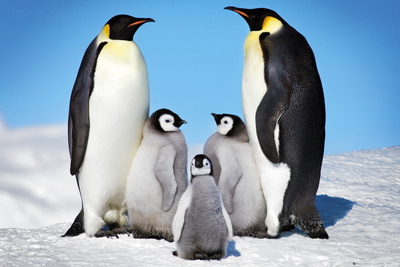
\includegraphics[scale=.50]{figures/Penguins.jpg}
\caption{TAMU figure - This is an example of a long figure title with a landscape figure.  Figure titles need to be single-spaced within and double spaced between in the list of figures.}
\label{fig:tamu-fig1-1}
\end{sidewaysfigure}
%%%%%%%%%%%%%%%%%%%%%%%%%%%%%%%%%%%%%%%%%%%%%%%%%%%%%%

More text here goes here.


Lorem ipsum dolor sit amet, consectetur adipiscing elit. Morbi augue urna, varius quis facilisis ac, imperdiet et nunc. Vestibulum ante ipsum primis in faucibus. 

\section{Testing the Top of the Page}
Maecenas accumsan lobortis dui fringilla suscipit. Quisque congue fringilla dui, sed eleifend sapien fringilla euismod. Pellentesque habitant morbi tristique senectus et netus et malesuada fames ac turpis egestas. Maecenas venenatis posuere magna quis tempus. Cras at leo massa, eu ultricies tellus. Nunc nec dictum augue. Cum sociis natoque penatibus et magnis dis parturient montes, nascetur ridiculus mus. Phasellus purus felis, mollis id scelerisque in, viverra in elit. Nulla iaculis ultrices justo, ac pharetra nisl rhoncus pulvinar. Duis vitae mauris velit, in congue massa.

Donec lectus orci, bibendum ut blandit dignissim, molestie non eros. Praesent aliquet feugiat dignissim. Morbi porttitor sollicitudin nisl, non mollis quam ultrices sit amet. Cras feugiat lacinia diam ut convallis. Nam nec varius ante. Nunc a ultrices felis. Quisque luctus sapien et ligula ornare quis consequat urna aliquet. Vestibulum vulputate lorem a tellus auctor id commodo risus sodales. Suspendisse quis tortor a felis molestie laoreet ut a nunc. Donec gravida sapien eget mauris condimentum lacinia. Proin eu purus libero. Nullam augue mi, vestibulum in convallis eu, adipiscing ac arcu. Donec nisi libero, egestas et molestie in, mollis quis ipsum. Sed gravida quam sit amet ante tempus rutrum non in mi. Cras viverra facilisis eros, id vestibulum sapien malesuada eget. Maecenas imperdiet luctus nisi vitae suscipit.



Aliquam erat volutpat. Integer ut mauris elit. Nam et lectus vel neque vehicula commodo. Integer at risus ligula. Fusce mollis mauris sed lorem aliquam bibendum porttitor tellus blandit. Curabitur enim nibh, accumsan eu elementum id, rutrum a ipsum. Vivamus ultricies, elit id ornare iaculis, metus justo posuere quam, sit amet bibendum arcu dolor a eros. Sed in nisl nibh. Aenean egestas est ut tortor volutpat vehicula. Maecenas aliquet placerat nunc hendrerit dictum. In et nisi massa. Pellentesque luctus, sapien quis dignissim vulputate, sapien libero bibendum velit, vitae auctor ipsum nulla at augue. Nulla ac eros vitae tortor elementum vehicula.

Morbi tristique egestas placerat. Cras faucibus eleifend porta. Class aptent taciti sociosqu ad litora torquent per conubia nostra, per inceptos himenaeos. Ut a pellentesque neque. Donec sollicitudin metus varius nulla egestas laoreet. Duis non mauris ut nunc adipiscing volutpat. Nam vitae est sed turpis tristique varius. 

\subsection{This is a Very Long Subsection Title This is a Very Long Subsection Title}

More text
\subsection{Subsection}

Subsection text

\section{Another Section}

Section text

%%%%%%%%%%%%%%%%%%%%%%%%%%%%%%%%%%%%%%%%%%%%%%%%%%%
%
%  New template code for TAMU Theses and Dissertations starting Fall 2012.  
%  For more info about this template or the 
%  TAMU LaTeX User's Group, see http://www.howdy.me/.
%
%  Author: Wendy Lynn Turner 
%	 Version 1.0 
%  Last updated 8/5/2012
%
%%%%%%%%%%%%%%%%%%%%%%%%%%%%%%%%%%%%%%%%%%%%%%%%%%%

%%%%%%%%%%%%%%%%%%%%%%%%%%%%%%%%%%%%%%%%%%%%%%%%%%%%%%%%%%%%%%%%%%%%%%%
%%%                           SECTION II
%%%%%%%%%%%%%%%%%%%%%%%%%%%%%%%%%%%%%%%%%%%%%%%%%%%%%%%%%%%%%%%%%%%%%%

\chapter{\uppercase {Literature Review: The Importance of Research Part Two- This is designed to test long titles in the TOC}}

Text goes here.

\section{New Section}
%%%%%%%%%%%%%%%%%%%%%%%%%%%%%%%%%%%%%%%%%%%%%%%%%%%%%%
\begin{figure}[H]
\centering
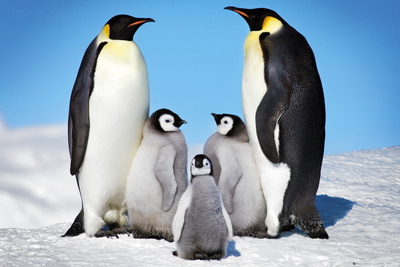
\includegraphics[scale=.50]{figures/Penguins.jpg}
\caption{TAMU figure - This is an example of a long figure title.  Figure titles need to be single-spaced within and double spaced between in the list of figures.}
\label{fig:landscapepenguins}
\end{figure}
%%%%%%%%%%%%%%%%%%%%%%%%%%%%%%%%%%%%%%%%%%%%%%%%%%%%%%
\subsection{Subsection}
\begin{table}[H]
\centering
\caption{This is a table template - This is an example of a long table title.  Table titles need to be single-spaced within and double spaced between in the list of tables.}
\begin{tabular}{|l|c|c|c|c|c|}
\hline
Product & 1 & 2 & 3 & 4 & 5\\
\hline
Price & 124.- & 136.- & 85.- & 156.- & 23.-\\
Guarantee [years] & 1 & 2 & - & 3 & 1\\
Rating & 89\% & 84\% & 51\% & & 45\%\\
\hline
\hline
Recommended & yes & yes & no & no & no\\
\hline
\end{tabular}
\label{tab:template1}
\end{table}


\subsection{Subsection}
%%%%%%%%%%%%%%%%%%%%%%%%%%%%%%%%%%%%%%%%%%%%%%%%%%%%%%
\begin{figure}[H]
\centering
\includegraphics[scale=.50]{figures/Sunset.jpg}
\caption{Sunset figure}
\label{fig:sunset-fig2}
\end{figure}
%%%%%%%%%%%%%%%%%%%%%%%%%%%%%%%%%%%%%%%%%%%%%%%%%%%%%%
\subsubsection{This is a subsubsection}
\begin{table}[H]
\centering
\caption{This is a table template - This is an example of a long table title.  Table titles need to be single-spaced within and double spaced between in the list of tables.}
\begin{tabular}{|l|c|c|c|c|c|}
\hline
Product & 1 & 2 & 3 & 4 & 5\\
\hline
Price & 124.- & 136.- & 85.- & 156.- & 23.-\\
Guarantee [years] & 1 & 2 & - & 3 & 1\\
Rating & 89\% & 84\% & 51\% & & 45\%\\
\hline
\hline
Recommended & yes & yes & no & no & no\\
\hline
\end{tabular}
\label{tab:template1-2}
\end{table}
\section{Another Section}

%%%%%%%%%%%%%%%%%%%%%%%%%%%%%%%%%%%%%%%%%%%%%%%%%%%
%
%  New template code for TAMU Theses and Dissertations starting Fall 2016.  
%
%
%  Author: Sean Zachary Roberson
%  Version 3.17.06
%  Last Updated: 6/15/2017
%
%%%%%%%%%%%%%%%%%%%%%%%%%%%%%%%%%%%%%%%%%%%%%%%%%%%
%%%%%%%%%%%%%%%%%%%%%%%%%%%%%%%%%%%%%%%%%%%%%%%%%%%%%%%%%%%%%%%%%%%%%%
%%                           SECTION III
%%%%%%%%%%%%%%%%%%%%%%%%%%%%%%%%%%%%%%%%%%%%%%%%%%%%%%%%%%%%%%%%%%%%%



\chapter{VERY, VERY, VERY LONG TITLE THAT FLOWS INTO A SECOND LINE FOR THE SAKE OF EXAMPLE}

Notice that the title of this section is long - much longer than the others. When you have long section titles, this template takes care of double spacing the lines in the title. If the title is long to fit in the table of contents, the template will single space the title.

\section{Yet Another Table}

Another table is placed here to show the effect of having tables in multiple sections. The list of tables should still double space between table titles, while single spacing long table titles.

%Fix table labeling.
\begin{table}[h!]
	\centering
	\begin{tabular}{|l|l|}
		\hline
		Dates & Attendance  \\ \hline
		August 8-10, 2008 & 3,523  \\ \hline
		August 14-16, 2009 & 4,003 \\ \hline
		July 9-11, 2010 & 5,049 \\ \hline
		August 5-7, 2011 & 6,891  \\ \hline
		August 10-12, 2012 & 9,464  \\ \hline
		August 16-18, 2013 & 11,077  \\ \hline
		July 18-20, 2014 & 14,686 \\ \hline
		July 31-August 2, 2015 & 18,411  \\ \hline
	\end{tabular}
	\caption{San Japan attendance. Data is taken from \cite{ANCONS}. I intentionally make the title of this table long so the single space effect is seen in the list of tables.}
\end{table}

You may be wondering why San Japan was chosen. There are a few reasons as to why I did this:

\begin{enumerate}
\item It is one of the fastest-growing anime conventions in Texas.
\item Filler.
\item I wanted a good variety of table examples.
\item Because conventions are cool.
\end{enumerate}

The \textit{enumerate} environment was used to generated an ordered list above.

\section{Section Test Example}
We insert another figure here, just for kicks.

\begin{figure}[h!]
	\centering
	\includegraphics[width = 6.0in]{LowPass_Filter_Design.png}
	\caption{A low pass filter design.}
\end{figure}

\subsection{Filler, Filler, Filler}

This section has filler text. These words serve no meaning except to fill a few lines in the document. This section has filler text. These words serve no meaning except to fill a few lines in the document. This section has filler text. These words serve no meaning except to fill a few lines in the document.

\begin{figure}[h!]
	\centering
	\includegraphics[width=3.75in]{Workspace1.png}
	\caption{A typical Texmaker workspace in Windows 7. The right sidebar displays the current file's structure according to the subsections in place.}
\end{figure}

This section has filler text. These words serve no meaning except to fill a few lines in the document. This section has filler text. These words serve no meaning except to fill a few lines in the document. This section has filler text. These words serve no meaning except to fill a few lines in the document. This section has filler text. These words serve no meaning except to fill a few lines in the document. This section has filler text. These words serve no meaning except to fill a few lines in the document. This section has filler text. These words serve no meaning except to fill a few lines in the document.

\begin{figure}[h!]
	\centering
	\includegraphics[width=3.5in]{Rachl1.png}
	\caption{Some commands in R.}
\end{figure}

\subsection{Subsection Test Example}
Test subsection for TOC display

\subsection{Subsection Test Example 2}
This section has filler text. These words serve no meaning except to fill a few lines in the document. This section has filler text. These words serve no meaning except to fill a few lines in the document. This section has filler text. These words serve no meaning except to fill a few lines in the document.

\begin{figure}[h!]
	\centering
	\includegraphics[scale=0.85]{TAM_Logo1.png}
	\caption{The logo of a familiar university.}
\end{figure}

\begin{figure}[!h]
	\caption{Yet another blank float that has no purpose. This is only to test the appearance of the Lists of Figures and the List of Tables.}
\end{figure}

\subsection{Section Summary}
  
This holds the summary. Well, not really a summary - there was a lot of filler in this section.

\begin{figure}[h!]
	\centering
	\includegraphics[width=6.5in]{Filter1.png}
	\caption{A signal and the result after a basic filter. The FFT was used to create the plot on the right.}
\end{figure}

\section{Section Test Example 3}
Test section for toc display only.

\begin{figure}[!h]
	\caption{There is nothing to see here.}
\end{figure}

\begin{figure}[!h]
	\caption{There is another float here. I wonder what could be here? Guess what? Nothing! There is no material in this float.}
\end{figure}

\subsection{Subsection Test 1}
Test subsection for toc display only.

\subsection{Subsection Test 2}
Test subsection for toc display only.


fix spacing in bibliography, if any...
%%%%%%%%%%%%%%%%%%%%%%%%%%%%%%%%%%%%%%%%%%%%%%%%%%%%%%%%%%%%%
\let\oldbibitem\bibitem
\renewcommand{\bibitem}{\setlength{\itemsep}{0pt}\oldbibitem}
%%%%%%%%%%%%%%%%%%%%%%%%%%%%%%%%%%%%%%%%%%%%%%%%%%%%%%%%%%%%%%%
%%%%%%%%%%%%%%%%%%%%%%%%%%%%%%%%%%%%%%%%%%%%%%%%%%%
%
%  New template code for TAMU Theses and Dissertations starting Fall 2012.  
%  For more info about this template or the 
%  TAMU LaTeX User's Group, see http://www.howdy.me/.
%
%  Author: Wendy Lynn Turner 
%	 Version 1.0 
%  Last updated 8/5/2012
%
%%%%%%%%%%%%%%%%%%%%%%%%%%%%%%%%%%%%%%%%%%%%%%%%%%%


%%%%%%%%%%%%%%%%%%%%%%%%%%%%%%%%%%%%%%%%%%%%%%%%%%%%%%%%%%%%%%%%%%%%%%
%%                           REFERENCES 
%%%%%%%%%%%%%%%%%%%%%%%%%%%%%%%%%%%%%%%%%%%%%%%%%%%%%%%%%%%%%%%%%%%%%

\phantomsection
\addcontentsline{toc}{chapter}{REFERENCES}

\renewcommand{\bibname}{{\normalsize\rm REFERENCES}}

\bibliographystyle{plain}
\bibliography{references}
% %%%%%%%%%%%%%%%%%%%%%%%%%%%%%%%%%%%%%%%%%%%%%%%%%%%
%
%  New template code for TAMU Theses and Dissertations starting Fall 2012.  
%  For more info about this template or the 
%  TAMU LaTeX User's Group, see http://www.howdy.me/.
%
%  Author: Wendy Lynn Turner 
%	 Version 1.0 
%  Last updated 8/5/2012
%
%%%%%%%%%%%%%%%%%%%%%%%%%%%%%%%%%%%%%%%%%%%%%%%%%%%

\begin{appendices}
\titleformat{\chapter}{\centering\normalsize}{APPENDIX \thechapter}{0em}{\vskip .5\baselineskip\centering}
\renewcommand{\appendixname}{APPENDIX}

%%%%%%%%%%%%%%%%%%%%%%%%%%%%%%%%%%%%%%%%%%%%%%%%%%%
%
%  New template code for TAMU Theses and Dissertations starting Fall 2012.  
%  For more info about this template or the 
%  TAMU LaTeX User's Group, see http://www.howdy.me/.
%
%  Author: Wendy Lynn Turner 
%	 Version 1.0 
%  Last updated 8/5/2012
%
%%%%%%%%%%%%%%%%%%%%%%%%%%%%%%%%%%%%%%%%%%%%%%%%%%%

%%%%%%%%%%%%%%%%%%%%%%%%%%%%%%%%%%%%%%%%%%%%%%%%%%%%%%%%%%%%%%%%%%%%%%
%%                           APPENDIX A 
%%%%%%%%%%%%%%%%%%%%%%%%%%%%%%%%%%%%%%%%%%%%%%%%%%%%%%%%%%%%%%%%%%%%%

\phantomsection

\chapter{\uppercase{First Appendix}}

Text for the Appendix follows.

\begin{figure}[H]
\centering
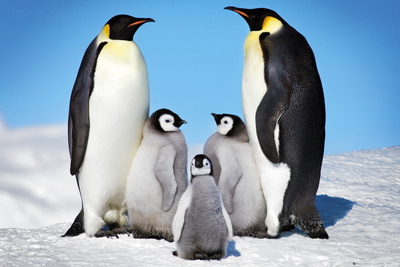
\includegraphics[scale=.50]{figures/Penguins.jpg}
\caption{TAMU figure}
\label{fig:tamu-fig5}
\end{figure}

%%%%%%%%%%%%%%%%%%%%%%%%%%%%%%%%%%%%%%%%%%%%%%%%%%%
%
%  New template code for TAMU Theses and Dissertations starting Fall 2016.
%
%
%  Author: Sean Zachary Roberson 
%	 Version 3.16.09 
%  Last updated 9/12/2016
%
%%%%%%%%%%%%%%%%%%%%%%%%%%%%%%%%%%%%%%%%%%%%%%%%%%%

%%%%%%%%%%%%%%%%%%%%%%%%%%%%%%%%%%%%%%%%%%%%%%%%%%%%%%%%%%%%%%%%%%%%%%
%%                           APPENDIX B
%%%%%%%%%%%%%%%%%%%%%%%%%%%%%%%%%%%%%%%%%%%%%%%%%%%%%%%%%%%%%%%%%%%%%

\chapter{\uppercase {A Second Appendix Whose Title Is Much Longer Than The First}}

Text for the Appendix follows.

\begin{figure}[h]
\centering
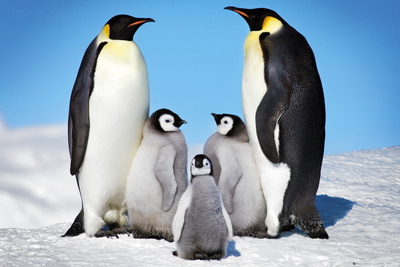
\includegraphics[scale=.50]{figures/Penguins.jpg}
\caption{Another TAMU figure.}
\label{fig:tamu-fig6}
\end{figure}

\section{Appendix Section}

\section{Second Appendix Section}


\pagebreak{}

\end{appendices}


\end{document}
